\begin{figure}[t!]
    \centering
    \begin{subfigure}[b]{\linewidth}
        \centering
        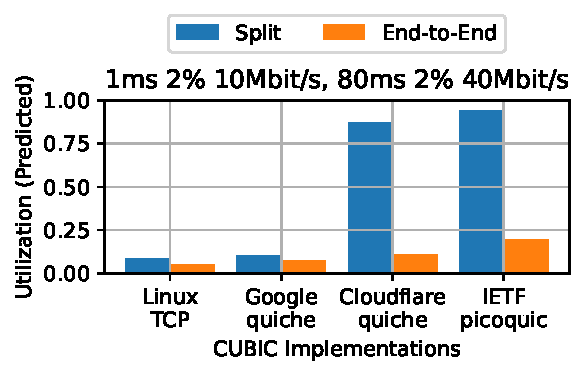
\includegraphics[width=0.8\linewidth]
         {figures/network_path_analysis/network_path_analysis_10_40_1_80_2_2.pdf}
        \captionsetup{skip=0pt}
        \caption{Some QUIC CUBIC implementations can benefit in new network
         classes where TCP CUBIC could not.}
        \label{fig:quic-predictions:cubic}
    \end{subfigure}
    \begin{subfigure}[b]{\linewidth}
        \centering
        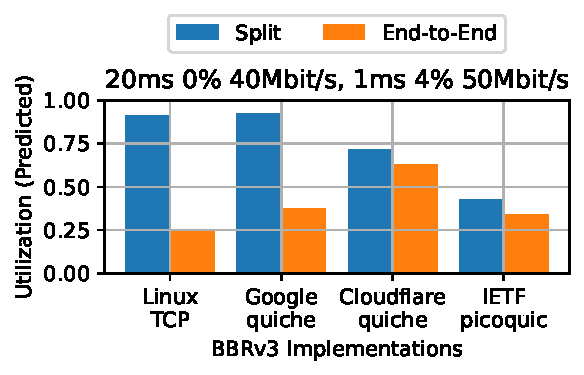
\includegraphics[width=0.8\linewidth]
         {figures/network_path_analysis/network_path_analysis_40_50_20_1_0_4.pdf}
        \captionsetup{skip=0pt}
        \caption{The various BBRv3 implementations have non-uniform end-to-end
         behavior and no clear resulting split behavior.}
        \label{fig:quic-predictions:bbr3}
    \end{subfigure}
    \caption{Predicted bottleneck link rate utilizations calculated from the
     predicted end-to-end and split throughputs of the TCP and QUIC
     implementations, on two different network path segments. End-to-end
     behavior of each CCA varies significantly by implementation.}
    \label{fig:quic-predictions}
    \vspace{-0.4cm}
\end{figure}
